%%%%%%%%%%%%%%%%%%%%%%%%%%%%%%%%%%%%%%%%%%%%%%%%%%%%%%%%%%%%%%%
% testbed.tex (part of thesis.tex)
% author: Qie Hu
%
%%%%%%%%%%%%%%%%%%%%%%%%%%%%%%%%%%%%%%%%%%%%%%%%%%%%%%%%%%%%%%%

% !TEX root = ../thesis.tex

\documentclass[../thesis.tex]{subfiles}
\begin{document}

\subsection{Testbed for System Identification}
We model the temperature evolution of the fourth floor of Sutardja Dai Hall (SDH), a building on the University of California, Berkeley campus. This floor contains offices for research staff and open workspaces for students, and is divided into six zones for modeling purposes (Figure \ref{fig:floor_plan}).

The building is equipped with a variable air volume (VAV) HVAC system that is common to 30\% of all U.S. commercial buildings \cite{VAV}. The system contains large supply fans which drive air through heat exchangers, cooling it down to a desired supply air temperature (SAT), and then distribute air to VAV boxes located throughout the building. There are 21 VAV boxes located on the fourth floor that govern the airflow to each room. In addition, the supply air may be reheated at the VAV box before entering the room. 
%Table \ref{tab:Zone_VAV} provides information about the mapping of the 21 VAV boxes to the zones they serve.
\begin{figure}[hbtp]
\centering
\vspace*{-0.4cm}
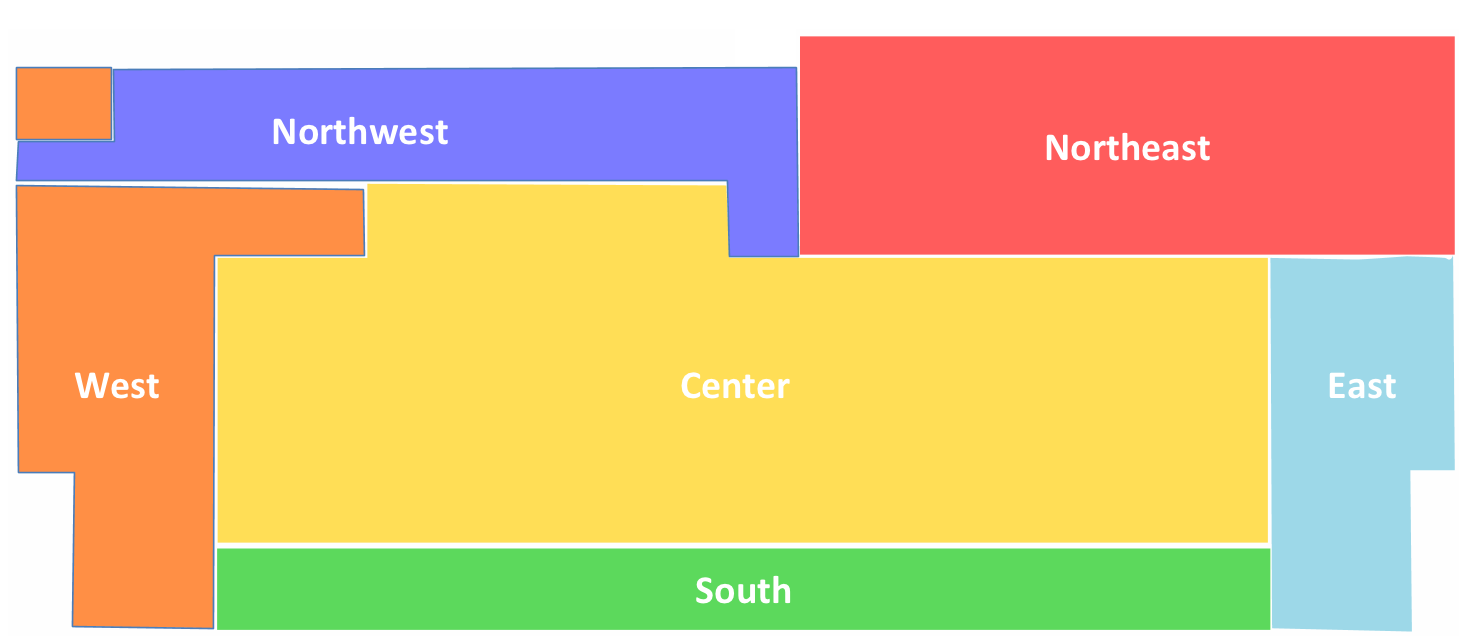
\includegraphics[scale=0.30]{chapters/building_model/figures/FloorPlan.png}
\vspace*{-0.05cm}
\caption{Zones for the 4th Floor of Sutardja Dai Hall (SDH)}
\label{fig:floor_plan}
\vspace*{-0.45cm}
\end{figure}

%\begin{table}[hbtp]
%\centering
%\begin{tabular}{*2c}
%\toprule
%Zone & VAV Boxes \\ \hline
%Northwest (NW) & 6, 8, 11 \\
%West (W) & 1, 2, 3 \\
%South (S) & 5, 9, 15, 16 \\
%East (E) & 20, 21 \\
%Northeast (NE) & 10, 14, 17, 19 \\
%Center (C) & 4, 7, 12, 13, 18 \\
%\bottomrule
%\end{tabular}
%\caption{VAV Boxes by Zone}
%\vspace*{-0.5cm}
%\label{tab:Zone_VAV}
%\end{table}

\end{document}